\section{Results and Analysis}

\label{results and analysis}

%Several factors impact the performance under \toolname:
%overhead of outlining and profiling, non-loop code, characteristics of applications, etc.
%In this section, we study these factors and compare the benefits of optimizing
%compilation using traditional coarse-grained random search (R), Fine-grained random search
%(FR), Greedy Combination (G), and Caliper-guided random search (CFR).
\begin{comment}
\subsection{Analysis of Overheads}
The outlining of hot loops into functions by Fine-grained Random Search (FR),
Greedy Combination (G), and Caliper-guided Random Search (CFR)
may affect inter-procedural
optimization (IPO).  Moreover, G and CFR rely on per-loop profiling
information to identify performant CVs.
%
Measurement overhead is inevitable in such scenarios due to
the use of instrumentation.  To
assess these costs, we compare the runtime of code variants subject to
such overhead with the baseline version and report the results in
\Cref{fig:overhead}.  We observe the following trends in these
results:

\vspace{.25em}
\noindent 1) Outlining hot loops typically introduces less than a 3\%
penalty on program performance across all architectures in our
experiments.
%, even though inter-module ipo is enabled by default for O3 baselines.
%The slowdowns on Intel Knights Landing (KNL) for LULESH is -22.5\%.
%We consider such a big slowdown as a performance bug of ICC/ICPC.
%Investigation of the root cause is out of this work's scope, thus we leave it as future work.
In fact, on AMD Opteron, we observe marginal performance improvements
for LULESH and AMG.
% Excluding the exceptional case of LULESH on KNL, we
Based on these results, we conclude that loop outlining can be done at
a low cost, which can often be offset by gains obtained using our
\toolname approach.

\vspace{.25em}
\noindent 2) Caliper instrumentation incurs less than 10\% slowdown
across all benchmarks and architectures.
% , but introduces 29.7\% and 18.1\% penalty to LULESH and Cloverleaf
% on KNL, respectively.  We suspect the slowdown of LULESH is due to
% the aforementioned ICC performance bug.  Slowdown of Cleverleaf can
% be attributed to two factors: the high synchronization overhead of
% KNL due to high number of threads and too many timing samples are
% taken for Cloverleaf (2.6X more than AMG because of more hot loops
% and invocations).
While reasonably low relative to the overall runtime, such a measurement
overhead can induce inaccuracy in the measured runtimes and
impact results of G and CFR.  We further discuss this issue in
\Cref{cv sensitivity,overallResults}.
\end{comment}

\begin{comment}
\begin{figure}
\includegraphics[width=\linewidth]{figures/sensitivity_opteron}
\caption{Benefit of Merged Non-Loop code CVs for CFR on AMD Opteron}
\label{fig:sensitivityOpteron}

\includegraphics[width=\linewidth]{figures/sensitivity_sandy}
\caption{Benefit of Merged Non-Loop code CVs for CFR on Intel Sandy Bridge}
\label{fig:sensitivitySandy}

\includegraphics[width=\linewidth]{figures/sensitivity_broadwell}
\caption{Benefit of Merged Non-Loop code CVs for CFR on Intel Broadwell}
\label{fig:sensitivityBroadwell}
\end{figure}
\end{comment}

\subsection{Sensitivity of Non-loop Code CVs}\label{cv sensitivity}

%Motivation
%As discussed, measurement error is calling for tolerance from
%\toolname search algorithms.
In our initial experiments, we found that even when the runtime spent in the
non-loop codes is a small fraction of the total runtime,
the choice of CVs for them can be vital to the overall performance
improvement.
Further, since we derive the non-loop runtime by subtracting the
runtimes of hot loops from the program end-to-end runtime, it also
includes the Caliper instrumentation overhead.  If this overhead is
much higher than the actual non-loop runtime, the derived non-loop
runtime may not be a good indicator for selecting the non-loop CVs
aimed at optimizing production runs that do not include Caliper
instrumentation. This issue may impact the performance improvements due to search
algorithms that rely on such information, i.e., CFR.

An alternative
metric to identify performant CVs for non-loop code is the program
end-to-end runtime since it is a good indicator of how non-loop and
hot-loop CVs interact.
Comparisons for CFR variants in \Cref{fig:sensitivity}
shows that, typically, both derived non-loop time (denoted
as \emph{Non-loop}) and end-to-end runtime (denoted as
\emph{Overall}) result in a significant performance improvement,
when used as the non-loop code runtime metric.  However, we obtain
 performance degradation in one case -- LULESH on Opteron -- if the
derived non-loop time metric is used.  Further, we find that
neither of these two metrics outperforms the other for all cases.
\vspace{2pt}
\begin{figure}
\centering
\subfloat[Comparison on AMD Opteron]{\includegraphics[scale=.4]
{gnuplot_temp/fc_opteron.pdf}
\label{fig:sensitivityOpteron}}
\subfloat[Comparison on Intel Sandy Bridge]{\includegraphics[scale=.4]
{gnuplot_temp/fc_sandy.pdf}
\label{fig:sensitivitySandy}}

\subfloat[Comparison on Intel Broadwell]{\includegraphics[scale=.4]
{gnuplot_temp/fc_broad.pdf}
\label{fig:sensitivityBroadwell}}
\vspace{-2mm}
\caption{Non-loop CV metrics: use of both derived non-loop runtime and overall runtime
metrics result in better performance.}
\label{fig:sensitivity}
\vspace{-4mm}
\end{figure}

These observations motivated us to combine the strength of the two metrics
(\emph{Non-loop} and \emph{Overall}) into one (denoted as
\emph{Merged} in \Cref{fig:sensitivity}), which concatenates the
top-30 best non-loop CVs from both \emph{Non-loop} and \emph{Overall}.
The concatenation results in 60 CVs for non-loop code, whereas only
the top-30 per-loop CVs are used for each hot loop.  Results in
\Cref{fig:sensitivity} show that \emph{Merged} delivers performance that
is either higher or close to the performance of \emph{Non-loop} and \emph{Overall}.  The reason for
this is that performant non-loop code CVs, which appear in both
\emph{Non-loop} and \emph{Overall} and are more likely to have a
positive performance impact, appear twice in \emph{Merged} and have a
higher probability of being used. Hence, in the remaining sections, we use
CFR to denote \emph{Merged} CFR.




\begin{figure*}
\subfloat[Part 1][Normalized speedups on AMD Opteron]
{\includegraphics[width=\linewidth]
{gnuplot_temp/opteron.pdf}
\label{fig:ro}}
\vspace{-1em}
\subfloat[Part 1][Normalized speedups on Intel Sandy Bridge]
{\includegraphics[width=\linewidth]
{gnuplot_temp/sandy.pdf}
\label{fig:rs}}
\vspace{-1em}
\subfloat[Part 1][Normalized speedups on Intel Broadwell]
{\includegraphics[width=\linewidth]
{gnuplot_temp/broad.pdf}
\label{fig:rb}}
%\vspace{-2mm}
\caption{CFR outperforms other methods for most cases: geometric mean of
speedups relative to the O3 baseline are 9.2\%, 10.3\%, and 9.4\% on
Opteron, Sandy Bridge, and Broadwell, respectively.}
\label{fig:results}
%\vspace{-2mm}
\end{figure*}


%results

%Caliper instrumentation usually incurs less than 5\% overhead.
% However, the overhead can be up to 30\% for Intel KNL many-core
% architecture due to high synchronization overhead.  Such high
% measurement overhead would dominate Caliper-based timing
% information, which makes CFR more important because its re-sampling
% and multiple-point evaluation can tolerate more measurement errors.
% However, we found even though non-loop code runtime is usually much
% smaller than total runtime of hot loops, its CVs plays a vital role
% in performance of the final binary.
\begin{comment}
\begin{figure}
\includegraphics[width=\linewidth]{figures/speedup_opteron}
\caption{Normalized Speedup for Lulesh, Cloverleaf and AMG on AMD Opteron}
\label{fig:ro}

\includegraphics[width=\linewidth]{figures/speedup_sandy}
\caption{Normalized Speedup for Lulesh, Cloverleaf and AMG on Intel Sandy Bridge}
\label{fig:rs}

\includegraphics[width=\linewidth]
{figures/speedup_broadwell}
\caption{Normalized Speedup for Lulesh, Cloverleaf and AMG on Intel Broadwell}
\label{fig:rb}
\end{figure}
\end{comment}



\begin{comment}
\begin{figure}
\includegraphics[width=\linewidth]
{figures/overall}
\caption{Normalized Speedups on AMD Opteron}
\label{fig:arch}

\includegraphics[width=\linewidth]
{figures/overall}
\caption{Normalized Speedups on Intel Sandy Bridge}
\label{fig:arch}

\includegraphics[width=\linewidth]
{figures/overall}
\caption{Normalized speedups on Intel Broadwell. G.realized is the
  actual speedup of Greedy algorithm while G.expected is the expected
  speedup of Greedy algorithm, calculated by summing up the best
  per-loop run times. FR and CFR are the two fine-grained search
  algorithms proposed by us, applied on the benchmarks with their hot
  loops outlined and without Caliper instrumentation; R is random
  search on per-program granularity, with the original unmodified
  benchmarks. }
\label{fig:arch}
\end{figure}
\end{comment}

%\begin{figure*}
%\includegraphics[width=\linewidth]
%{figures/overall}
%\caption{Normalized speedups on Intel Sandy Bridge}
%\label{fig:arch}
%\end{figure*}

%\begin{figure*}

%\end{figure*}

\subsection{Overall Performance Comparison} \label{overallResults}

Performance results for our benchmarks on the three
architectures are shown in \Cref{fig:results}. In this figure, R is coarse-grained
random search (\Cref{fig:csr}) for the original unmodified benchmarks,
FR (\Cref{alg:fr}) and CFR (\Cref{alg:cfr}) are the two fine-grained search
algorithms proposed by us, G.realized is the observed speedup of
the Greedy algorithm (\Cref{alg:greedy}), and G.expected is the
theoretical expected speedup of the Greedy algorithm calculated by
summing up the best per-loop and non-loop runtimes, which serves as
an analytical upper bound. FR, CFR, G.realized, and G.expected are all
applied on the benchmarks with their hot loops outlined and without Caliper
instrumentation.
%with detailed performance statistics presented in \Cref{table:stdO,table:stdS,table:stdB}.
From these results, we make the following observations.

\vspace{.25em}
\noindent 1) CFR provides the best performing executables for most
scenarios across benchmarks and architectures. It provides 9.2\%,
10.3\%, 9.4\% geometric mean speedups for Opteron, Sandy
Bridge and Broadwell, respectively.  It also achieves the best case
improvement of 18.1\% for AMG on AMD Opteron (see \Cref{fig:ro}) in
comparison to the O3 baseline.  In contrast, the performance
improvement due to R is only 3.4\%, 5.0\%, 4.6\% on the same
respective architectures.  In certain cases, R does not improve performance at all
while CFR does much better, e.g., for AMG on Sandy Bridge and
Broadwell.
% The gap is less on KNL, which may be due to misleading of high
% measurement error for runtimes.  Note that even though loop
% outlining incurs 22.5\% slowdown for LULESH, compared to O3
% baseline, CFR still performs 2.8\% better than R, which is already
% 37.7\% better than the baseline.

\vspace{.25em}
\noindent 2) G.realized results in significant slowdowns for many benchmark and
architecture combinations.  Although it improves performance of AMG on
Opteron and Sandy Bridge, the improvement is still inferior to that of
CFR.

\vspace{.25em}
\noindent 3) FR's performance is inferior to CFR and has high
variance.  For example, it achieves less than a 3\% improvement for
Cloverleaf on Opteron, Sandy Bridge and Broadwell, while CFR achieves
13.6\%, 15.2\% and 12.7\%, respectively.
%Even worse, it degrades Cloverleaf performance by 25.8\% on KNL.

The above comparison between R and CFR confirms our hypothesis that
fine-grained per-loop compilation can improve
program performance beyond that of a traditional per-program compilation model.
A comparison with FR indicates that the \toolname
approach of flag selection based on observed per-loop timings is
critical for performance improvement.  Finally, poor results for G.realized indicate
that greedily picking the best CVs for each hot-loop and non-loop code
is not sufficient. %Instead, CFR's multi-step, profile-guided approach
%is needed to get higher performance.
\vspace{-2mm}
\subsection{Comparison to the State-of-the-art} \label{beatPGO}

To meet the objective of compiler flag selection for each hot loop and
thus specialize compilation for a specific application, several prior
search-based and machine learning-based approaches exist.  As a
search-based approach, FuncyTuner optimizes each new program by
searching the COS for performant CVs from scratch.  The
state-of-the-art search algorithm in~\cite{cere} performs a
fine-grained flag selection for hot code regions and generates the
final executable in a greedy fashion, similar to G.realized in our
work.  Our results in \Cref{fig:results} show that
this degrades performance for several benchmarks for the Intel compiler tool chain.

COBAYN~\cite{cobayn}, a state-of-the-art machine
learning-based approach, infers performant CVs for a new program by
extracting static and dynamic program features and providing them as inputs to a
pre-trained Bayesian network.  To compare FuncyTuner with COBAYN, we
first train COBAYN on Intel Broadwell with cBench~\cite{cbench}.
Specifically, we select the top 100 performant CVs out of 1000 random
CV samples for each cBench application to extract their static and
dynamic features with Milepost-gcc~\cite{milepostgcc} and
Mica~\cite{mica}, respectively.  We then train three models,
{\em static, dynamic, and hybrid}, using static features, dynamic features
and all features, respectively.  Since COBAYN can only
perform inferences on binary compiler flags, we turn each multi-valued
ICC flag into a binary one by allowing it to have two values.  Then,
we use each of the three COBAYN models to generate 1000 CVs to compile
1000 code variants. The fastest code variant is considered as the
result of each model.  This comparison is fair, since both FuncyTuner
and COBAYN pick the best variant using information derived from data on 1000  variants.
\begin{figure*}
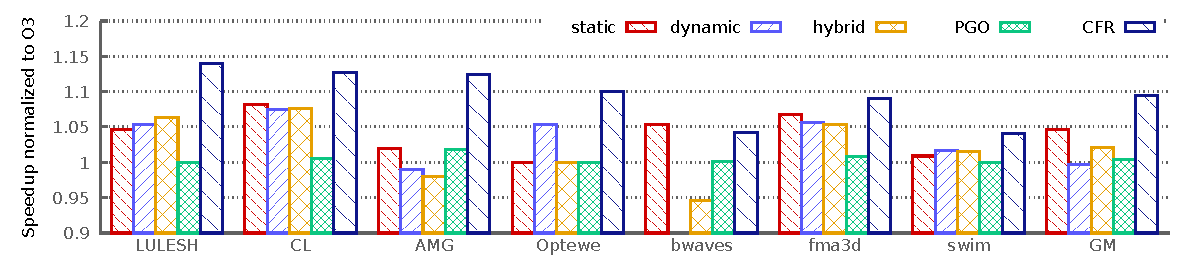
\includegraphics[width=\linewidth]{gnuplot_temp/pgo.pdf}
\vspace{-6mm}
\caption{FuncyTuner provides better performance than all variants of COBAYN(static, dynamic, hybrid) and PGO.}
\label{fig:pgo}
\vspace{-2mm}
\end{figure*}
%PGO results will be put here, together w/ COBAYN
%Figure needs to be redrawn
Both search-based approaches, FuncyTuner and COBAYN (and machine-learning techniques in general), take runtimes of different code variants as inputs.  However, runtimes are
only one of many program performance profile considerations.  In fact,
Intel compilers support built-in profile-guided
optimization~\cite{pgo} (PGO), which utilizes an instrumentation run
of a target program to collect profile information, such as loop trip
counts and indirect function call targets.  Therefore, the comparison
to PGO offers a perspective to evaluate the trade-off between benefits
and complexities for all approaches.  For a fair comparison, we use
"-qopenmp -fp-model source -prof-gen -prof-dir/app" for an
instrumented compilation (see recommendations for PGO in Intel's
compiler optimization manual) and then run the programs with tuning
inputs in \Cref{settings}.  Afterward, the programs are recompiled
with ``-O3 -qopenmp -fp-model source -prof-use -prof-dir/app''.

\begin{comment}
\begin{figure*}
\includegraphics[width=\linewidth]{gnuplot_temp/broad.pdf}
\caption{Normalized Speedup for Lulesh, Cloverleaf and AMG on AMD Opteron}
\label{fig:ro}
\end{figure*}
\end{comment}

\begin{comment}
\begin{figure}
\includegraphics[width=\linewidth]{gnuplot_temp/cobayn_compare.pdf}
\caption{FuncyTuner provides better performance than all variants of
    COBAYN (static, dynamic, hybrid).}
\label{fig:cobayn}
\end{figure}
\end{comment}

Results are shown in \Cref{fig:pgo}. Specifically, we make the following observations:

\noindent (1) COBAYN's static and hybrid models perform
4.6\% and 2.1\% (geometric mean) better than the O3 baseline, respectively,
while COBAYN's dynamic model is worse than the O3 baseline.
In contrast, FuncyTuner CFR improves performance by 9.4\% beyond the O3 baseline and outperforms COBAYN significantly.
  The
performance of COBAYN's static model is consistent with the findings
in the work that proposed COBAYN~\cite{cobayn} and other previous
research~\cite{1611549,Cavazos:2007:RSG:1251974.1252540,FursinMGL15}.
These related works also show that
a machine learning-based approach is able to reduce search overhead but
does not perform better than traditional random search ("Random" in our
paper) when the sample size is sufficiently large, e.g., 1000 samples.
The poor performance of COBAYN's dynamic and hybrid models may be
attributed to limited dynamic features, since MICA~\cite{mica} only
works with serial code while our target benchmarks are parallel.
% We also want to point out that FuncyTuner has little overhead to be
% ported onto different machines, while the re-training overhead can
% be prohibitively high for COBAYN.  As an example, extracting dynamic
% features for cBench takes around 2 days on a 16-node Broadwell
% cluster.

\noindent (2) PGO result in only minor performance improvements
relative to O3 and is inferior to \toolname CFR.  While PGO is 1.8\%
better than O3 for AMG, it shows little improvement on six other
programs.  In fact, PGO instrumentation runs fail for LULESH and
Optewe. 
%, and we consider its performance identical to O3. --> Frank:
%Dont say that, and don't report something you did nto measure!

In brief, \toolname delivers significantly better performance than
state-of-the-art techniques on our modern scientific simulation codes.
It only relies on Caliper light-weight source-code level
instrumentation \cite{caliper}, entailing much less engineering
complexities than both COBAYN and PGO.  Such simplicity is extremely
noticeable when one considers the fact that Intel compilers are
industry-quality production compilers and tuned for several decades,
and COBAYN depends on a variety of large tools, such as Milepost GCC
\cite{milepostgcc} and Mica.  Nevertheless, their performance is
inferior to \toolname and their robustness is limited.

\iffalse
\begin{figure}
\includegraphics[width=\linewidth]{figures/speedup_knl}
\caption{Net Speedup for Lulesh, Cloverleaf and AMG2013 on
    Intel Knights Landing}
\label{fig:rk}
\end{figure}
\fi

\begin{comment}
\begin {table}
%\nocaptionrule
\caption{Performance Statistics on Intel Broadwell}
\label{table:stdB}
%\vspace{2pt}
\centering
\resizebox{\columnwidth}{!}{%
\begin{tabular}{l|l|l|l|l|l|l }
\hline
%  & \\
\multirow{2}{*}{\textbf{Algorithm}} &  \multicolumn{2}{c|}{\textbf{Lulesh}} & \multicolumn{2}{c|}{\textbf{Cloverleaf}} & \multicolumn{2}{c}{\textbf{AMG}} \\
\cline{2-7}
 & \textbf{Mean} & \textbf{stdev} & \textbf{Mean} & \textbf{stdev} & \textbf{Mean} & \textbf{stdev} \\
\hline
%  & \\
G.expected & 10.9   & N/A & 5   & N/A & 11.8  & N/A\\
\hline
G.realized & 21.52 & 1.4 & 8.92 & 0.29 & 13.19 & 0.65 \\
\hline
O3.origin & 13.57 & 0.04 & 5.82 & 0.07 & 12.91 & 0.29 \\
\hline
O3.caliper & 13.91 & 0.05 & 5.91 & 0.08 & 13.4 & 0.48\\
\hline
O3.outlined & 13.82 & 0.04 & 5.79 & 0.06 & 12.97 & 0.48\\
\hline
R & 12.66 & 0.07 & 5.37 & 0.04 & 12.68 & 0.1 \\
\hline
FR & 12.76 & 0.07 & 5.7 & 0.05 &11.24 & 0.06\\
\hline
CFR & 12.11 & 0.42 & 5.05 & 0.04 & 11.3 & 0.08\\
\hline
\end{tabular}
}
\end {table}

\begin {table}
%\nocaptionrule
\caption{Performance Statistics on Intel Sandy Bridge}
\label{table:stdS}
%\vspace{2pt}
\centering
\resizebox{\columnwidth}{!}{%
\begin{tabular}{l|l|l|l|l|l|l }
\hline
%  & \\
\multirow{2}{*}{\textbf{Algorithm}} &  \multicolumn{2}{c|}{\textbf{Lulesh}} & \multicolumn{2}{c|}{\textbf{Cloverleaf}} & \multicolumn{2}{c}{\textbf{AMG}} \\
\cline{2-7}
 & \textbf{Mean} & \textbf{stdev} & \textbf{Mean} & \textbf{stdev} & \textbf{Mean} & \textbf{stdev} \\
\hline
%  & \\
G.expected & 5.7  & N/A & 3.7 & N/A & 6.1 & N/A\\
\hline
G.realized & 9.3 & 0.16 & 6.38 & 0.22 & 5.91 & 0.03 \\
\hline
O3.origin & 7.22 & 0.05 & 4.63 & 0.01 & 6.64 & 0.17 \\
\hline
O3.caliper & 8.0 & 0.05 & 4.76 & 0.04 & 7.4 & 0.3\\
\hline
O3.outlined & 7.39 & 0.08 & 4.65 & 0.03 & 6.66 & 0.13\\
\hline
R & 6.31 & 0.17 & 4 & 0.02 & 6.58 & 0.18 \\
\hline
FR & 6.24 & 0.12 & 4.54 & 0.03 &5.94 & 0.04\\
\hline
CFR & 6.19 & 0.18 & 3.9 & 0.01 & 5.78 & 0.02\\
\hline
\end{tabular}
}
\end {table}

\begin {table}
%\nocaptionrule
\caption{Performance Statistics on AMD Opteron}
\label{table:stdO}
%\vspace{2pt}
\centering
\resizebox{\columnwidth}{!}{%
\begin{tabular}{l|l|l|l|l|l|l }
\hline
%  & \\
\multirow{2}{*}{\textbf{Algorithm}} &  \multicolumn{2}{c|}{\textbf{Lulesh}} & \multicolumn{2}{c|}{\textbf{Cloverleaf}} & \multicolumn{2}{c}{\textbf{AMG}} \\
\cline{2-7}
 & \textbf{Mean} & \textbf{stdev} & \textbf{Mean} & \textbf{stdev} & \textbf{Mean} & \textbf{stdev} \\
\hline
%  & \\
G.expected & 9.7  & N/A & 5.73 & N/A & 9.4 & N/A\\
\hline
G.realized & 14.52 & 0.37 & 11.01 & 0.15 & 9.6 & 0.07 \\
\hline
O3.origin & 11.1 & 0.08 & 6.88 & 0.16 & 10.27 & 0.25 \\
\hline
O3.caliper & 11.05 & 0.05 & 7.38 & 0.09 & 10.99 & 0.62\\
\hline
O3.outlined & 10.84 & 0.03 & 6.89 & 0.14 & 10.13 & 0.25\\
\hline
R.origin & 10.87 & 0.08 & 6.96 & 0.12 & 10.19 & 0.37 \\
\hline
FR & 10.27 & 0.05 & 6.7 & 0.07 & 9.73 & 0.92 \\
\hline
CFR & 10.16 & 0.05 & 6.06 & 0.08 & 8.7 & 0.27\\
\hline
\end{tabular}
}
\end {table}
\end{comment}

\iffalse
\begin {table}[!htb]
%\nocaptionrule
\caption{\textbf{Performance Statistics on Intel KNL}}
\label{table:stdK}
%\vspace{2pt}
\centering
\resizebox{\columnwidth}{!}{%
\begin{tabular}{l|l|l|l|l|l|l }
\hline
%  & \\
\multirow{2}{*}{\textbf{Algorithm}} &  \multicolumn{2}{c|}{\textbf{Lulesh}} & \multicolumn{2}{c|}{\textbf{Cloverleaf}} & \multicolumn{2}{c}{\textbf{AMG}} \\
\cline{2-7}
 & \textbf{Mean} & \textbf{stdev} & \textbf{Mean} & \textbf{stdev} & \textbf{Mean} & \textbf{stdev} \\
\hline
%  & \\
G.expected & 6  & N/A & 6.2 & N/A & 8.74 & N/A\\
\hline
G.realized & 6.81 & 0.01 & 5.13 & 0.01 & 9.75 & 0.02 \\
\hline
O3.origin & 6.87 & 0.11 & 5.31 & 0.01 & 9.28 & 0.01 \\
\hline
O3.caliper & 9.77 & 0.04 & 6.48 & 0.01 & 9.64 & 0.03\\
\hline
O3.outlined & 8.87 & 0.02 & 5.33 & 0.01 & 9.29 & 0.05\\
\hline
R & 4.99 & 0.01 & 5.32 & 0.01 & 8.85 & 0.01 \\
\hline
FR & 5.82 & 0.01 & 7.16 & 0.02 &9.15 & 0.02\\
\hline
CFR & 4.89 & 0.01 & 5.12 & 0.01 & 8.83 & 0.03\\
\hline
\end{tabular}
}
\end {table}
\fi

\subsection{Impact Of Different Inputs} \label{inputsensitivity}
\begin{figure}
\centering
\includegraphics[width=0.6\textwidth]{gnuplot_temp/scale_CL.pdf}
%\vspace{-5mm}
\caption{For Cloverleaf on Broadwell, FuncyTuner CFR provides stable performance benefit than all others while scaling from 100 to 800 time-steps.}
\label{fig:cl}
%\vspace{-5mm}
\end{figure}

\begin{figure*}
\subfloat[Part 1][Normalized speedups for small inputs]
{\includegraphics[width=\linewidth]
{gnuplot_temp/small.pdf}
\label{fig:small}}
\vspace{-1em}
\subfloat[Part 1][Normalized speedups for large inputs]
{\includegraphics[width=\linewidth]
{gnuplot_temp/large.pdf}
\label{fig:large}}
\vspace{-2mm}
\caption{CFR shows little performance sensitivity on small and large inputs with geometric mean of speedups relative to the O3 baseline 12.3\% and 10.7\% respectively.}
\vspace{-4mm}
\label{fig:sensitivity}
\end{figure*}
The over-arching goal of our work is to auto-tune large scientific
simulation codes with a given input.  Such inputs capture the sizes of
work sets in practice, hence, their performance generalizes to other
inputs as we will show, e.g., for inputs with the same work-set size
but different simulation time-steps. This is shown in
\Cref{fig:cl} for Cloverleaf on Broadwell by varying number of
time-steps as part of the input.
\begin{comment}
\begin {table}[t]
%\nocaptionrule
\caption{Small and large inputs. Format}
%\vspace{2pt}
\centering
{\footnotesize
\label{table:apps}
\begin{tabular}{ p{1.7cm}p{2.0cm}p{1.7cm}}
%\hline
%  & \\
\textbf{Name} & \textbf{Small} & \textbf{Large}\\
\hline
AMG & 20 & 30 \\ \hline
LULESH & 180& 250\\ \hline
Cloverleaf (CL) & 1000 & 4000\\ \hline
351.bwaves & test & ref \\ \hline
362.fma3d & test & ref \\ \hline
363.swim & test & ref \\ \hline
Optewe & 384& 768\\ \hline
\end{tabular}
}
\end {table}
\end{comment}

\begin{comment}
\begin {table}[t]
%\nocaptionrule
\caption{List of benchmarks. LOC: lines of source code.}
%\vspace{2pt}
\centering
{\footnotesize
\label{table:apps}
\begin{tabular}{ p{1.7cm}p{2.0cm}p{3.4cm}}
%\hline
%  & \\
\textbf{Name} & \textbf{Small} & \textbf{Large}\\
\hline
AMG & 20 & 30 \\ \hline
LULESH & 180,10 & 250,5 \\ \hline
Cloverleaf (CL) & (1000,300) & (4000,10)\\ \hline
351.bwaves & test (5, 150) & ref (160, 10) \\ \hline
362.fma3d & test (1, 8000) & ref (END=1.5E-4, END=1.5E-6) \\ \hline
363.swim & test (10, 20000) & ref (3000, 50) \\ \hline
Optewe & 384, 15 & 768, 1\\ \hline
\end{tabular}
}
\end {table}
\end{comment}

Inputs with different work-set sizes are addressed as follows.  We
experimented on Broadwell with two sets of inputs that have different
input sizes from those in \Cref{settings}. For 351.bwaves, 362.fma3d,
and 363.swim, we use ``test'' and ``ref'' as their small and large
inputs, respectively. For LULESH, AMG, Cloverleaf, Optewe, their small
input sizes are 180, 20, 1000, 384, respectively, while their large
input sizes are 250, 30, 4000, 768, respectively.  As shown in
\Cref{fig:sensitivity}, we observe little sensitivity for these small
and large inputs, except that for 351.swim \toolname CFR does not
perform as well as the other three approaches for its small
input. Nonetheless, CFR for 351.swim is still 20.6\% better than PGO and the
O3 baseline.  We attribute such performance to the fact that the
``test'' input is so small that each time-step takes less than .01
seconds, which significantly differs from the performance profile of its
tuning input.
%In fact, the instrumentation overhead is 41.2\% high of its O3 baseline. 
However, such a small input rarely exists in practice and is not our
primary focus.

%{\bf Why is the following commented out? Check the latex source! Is
%  this intentional?} Answer by Tao {Yes. The commented one was the first draft I had, not usable anymore.}
\begin{comment}
In our experimental settings, we verify that this is true with O3 baseline when we conduct the input size reduction.
We further verify this property on Intel Broadwell with inputs different from the tuning inputs.
%
These inputs are selected according to the following two
guidelines: 1) Increase the time-steps for tuning-inputs, and 2) increase
the input scales.

Our experiments show that on the inputs of interest to scientific
simulation codes, there is little input sensitivity and the tuning
performance benefits can generalizes beyond the training inputs.
\end{comment}
%A prior work \cite{Chen:2010:EIO:1806596.1806647} by Chen et al. validates that search-based tuning has limited input sensitivity across 1000 inputs on their benchmark suite.
%To the best of our knowledge, there is no guideline to select inputs so that they will capture different work sets automatically.


\vspace{-1ex}
\subsection{Deep Dive: Cloverleaf On Broadwell} \label{case-study}

% Furthermore, CFR evaluates 1000 MCVs re-sampled from the per-loop
% compressed CV sample space in contrast to G, which only evaluates
% one MCV. This enables CFR to learn from diverse interactions among
% different CVs and compilation modules to obtain higher performing
% executables.  To gain further insights, we conduct an in-depth case
% study for Cloverleaf on Intel Broadwell.  motivation

\subsubsection{\textbf{Design}}

Broadly speaking, CFR utilizes per-loop runtime
information to direct the fine-grained search towards better
performing CVs.  Insights about the performance characteristics of
different algorithms compared in this paper can be useful for further
improving program performance.  Specifically, we want to answer the
following two questions:
%Thus, we carry out a case study to answer the following two questions:
\begin{itemize}
\item \textbf{$Q_1$}: Why does G.realized often introduce slowdowns
  while expected to have performance improvements?
\item \textbf{$Q_2$}: Why does CFR perform better than others?
\end{itemize}

% approach To this end, we perform an in-depth analysis of Cloverleaf
% on Intel Broadwell.
To this end, we select Cloverleaf to perform an in-depth case study on
Intel Broadwell due to the following considerations: first, its
non-loop code is written in Fortran, and hot loops are in C.  This may
provide more challenges and opportunities for ICC's inter-procedural
optimizations (IPO).  Second, its hot loops have simple source code
structures, e.g., they neither feature control flow nor deep loop
nests, thus presenting opportunities for ICC to perform optimizations
related to loop unrolling and vectorization, which often have a
significant impact on program performance.
% and are friendly for manual inspection of generated code to
% understand how they have been performed.
Five hot loops of Cloverleaf are selected since they have
comparatively high per-loop runtime ratios (see \Cref{table:study},
others are less than 3.0\%) and were found to produce large
performance differences (see \Cref{fig:case}) across different
tuning algorithms.
%, which provides more opportunities to interpret them with Likwid fine-grained profiling data~\cite{likwid}.

%more about approach: greedy reduction
Since each CV has more than 30 flags, it is difficult to identify
performance-critical flags in the best CVs chosen by different algorithms.
We use a greedy
algorithm to eliminate the flags that have low impact on the
program runtime.  The algorithm tries to eliminate one
flag for a specified loop CV (\emph{focused CV}) while
keeping all other CVs intact.  If excluding a flag from \emph{focused
  CV} does not degrade program performance, the flag is removed;
otherwise, it is kept intact.  This process is performed iteratively until no more
flags of \emph{focused CV} can be eliminated.  We consider the remaining flags in
\emph{focused CV} as the critical ones for the given loop.
Note that we only consider the static COBAYN model, because it is
superior to its dynamic and hybrid counterparts for Cloverleaf.
% Let's denote the flag being considered as $F_c$
%
% If there is no performance degradation while excluding the flag under
% consideration from then After one iteration of evaluating flags of
% the given CV, it keeps all flags that contribute to performance
% improvements (i.e., if such a flags were to be removed, performance
% would drop).  without performance degradation, which guarantees that
% the reduced CVs produce a binary with similar runtime (within 1\%
% difference).  This enables us to reason which flags are critical for
% a compilation module of interest.

\begin {table}
%\nocaptionrule
  \caption{Critical flags for Cloverleaf. O3 is always included in the CV.}
  \vspace{-3mm}
\label{table:algs}
\small
\centering
\begin{tabular}{ l|l|l }
%\hline
%  & \\
\textbf{Algorithm} & \textbf{Loop} & \textbf{Flags} \\
\hline
R/COBAYN & all &-qopt-streaming-stores=always\\
 & &-no-ansi-alias -ipo -xCORE-AVX2 \\
\hline
CFR& dt & -no-vec\\
\hline
CFR& cell3 & none\\
\hline
CFR& cell7 & none\\
\hline
CFR& mom9 & -no-vec\\
\hline
G.realized & mom9 & none \\
\hline
\end{tabular}
\vspace{-4mm}
\end {table}


\subsubsection{\textbf{Observations}}

%results and observation
\Cref{fig:case} shows the per-loop normalized performance
improvement due to G.realized, R/COBAYN, CFR, and G.expected for the five Cloverleaf
hot loops on Broadwell.  After greedy
elimination, the COBAYN static model has the same critical flags as those
of R, and thus they share the same results.  \Cref{table:study} reveals which critical
optimizations, such as loop unrolling and vectorization, are exploited by
different algorithms in this case.
\begin{comment}

Unless explicitly mentioned, there is no
loop unrolling.  Here, unroll2 and unroll3 indicate unroll twice and
three times, respectively.  There is no vectorization (scalar) by
default.  Broadwell has a 256-bit width SIMD unit.  With
``-xCORE-AVX2'', ICC can choose 128-bit or 256-bit SIMD instructions
for vectorization.  128-vec vectorizes a loop with 128-bit simd
instructions while 256-vec may use both 128-bit and 256-bit simd
instructions. \emph{RS} has register-spilling instructions.  \emph{IO}
means that instruction scheduling order is different from the one
without IO but with same notations, e.g., neither CFR nor G.realized
vectorizes Cloverleaf dt loop, but their generate code with different
instruction ordering.  \emph{IS} indicates that different instructions
are selected.  For example, both G.realized and R vectorizes loop
mom9, but instructions are different.
%, by inspecting the assembly code of binaries generated by them.
\end{comment}
We make the following observations:

\vspace{.25em}
\noindent (1) Vectorization is not always profitable. First, cell3
  and cell7 experience a 27.7\% and 13.6\% slowdown, respectively,
  when 256-bit vectorization is performed for R.  Other
  algorithms feature similar performance benefits, yet they do not
  vectorize.  Also, O3 uses 128-bit SIMD (single instruction multiple data) instructions.  Second, even though dt achieves a 34.8\%
  speedup with 256-bit vectorization, the performance improvement is
  still 12.8\% worse than a non-vectorized/scalar version. 
%
  Inspection of assembly code shows that there are many data permutations
  and mask operations to handle control flow divergence, which are
  known to degrade vectorization efficiency. Shorter loop trip counts
  caused by loop unrolling and OpenMP work sharing also
  contribute to the inferior performance of the vectorized loops.
\begin {table}
%\nocaptionrule
\caption{Comparison of optimizations for 5 Cloverleaf
kernels on Broadwell. scalar: not vectorized; \{128,256\}-vec: vectorized with
\{128,256\}-bit SIMD; unroll\{2,3\}: unroll 2/3 times; IO: instruction reordering;
IS: instruction selection; RS: register spilling.
}
\vspace{-2mm}
\label{table:study}
%\vspace{2pt}
\centering
%\resizebox{\columnwidth}{!}{%
\begin{tabular}{l|l|l|l|l|l }
\hline
%  & \\
\multirow{2}{*}{\textbf{Algorithm}} &  \multicolumn{5}{c}{\textbf{Kernel, O3 runtime ratio \%}} \\
\cline{2-6}
 & \textbf{dt, 6.3} & \textbf{cell3, 2.9} & \textbf{cell7, 3.5} & \textbf{mom9, 3.5} &\textbf{acc,  4.2} \\
%  & 6.3 & 2.9 & 3.5 & 3.5 & 4.2  \\
\hline
G.realized & scalar, IO & scalar & scalar & 256-vec, unroll2 &256-vec, IS, IO\\
%&IO & & & unroll2 &IS, IO\\
\hline
G.expected & scalar, RS, IO & scalar & scalar & scalar, IS & 256-vec \\
% & &  &  & IS &  \\
\hline
O3.origin & scalar, unroll2 & scalar & scalar & 128-vec & scalar, unroll3\\
%&  & & & &\\
\hline
R (COBAYN static)& 256-vec & 256-vec & 256-vec & 256-vec, IS &256-vec, IS\\
% &  &  &  & IS &IS\\
\hline
CFR & scalar & scalar & scalar & scalar, IS& 256-vec\\
% &  &  &  & IS &\\
\hline
\end{tabular}
%}
\vspace{-4mm}
\end {table}

\vspace{.25em}
\noindent (2) G.realized performs worse than other algorithms.
With different per-loop CVs from those of G.expected, IPO decisions are subject to changes. For example, G.realized vectorizes mom9 with 256-bit AVX2 instructions and further unrolls the vectorized loop twice while G.expected does not. In contrast, \toolname CFR has more informed freedom to select non-conflicting CVs. e.g., it selects "-no-vec" for mom9 to avoid vectorization.
%since IPO can invalidate decisions made earlier by local per-loop  cost
%  models.  For example, G.realized vectorizes mom9 with 256-bit AVX2
%  instructions and further unrolls the vectorized loop twice while
%  G.expected does not.
%  In contrast, CFR alleviates the conflict that G.realized experiences with IPO by
%  sampling more CVs in $COS_{new}$ with Caliper's guidance.
%  In fact, CFR selects a CV which does not use IPO for mom9.
  
  %so that it is able to find out CVs which have fewer conflicts.
  %\textbf{(How does more sampling concretely alleviate this? What are
  %  the flag differences??? Too vague, could backfire. Can you verify
  %  that CFR does not include IPO in this case? If so, mention it here.)}

\vspace{.25em}
\noindent (3) Other optimizations, such as instruction scheduling (IO), register
  allocation (RS), loop unrolling (unroll), and instruction selection (IS), also
  matter, e.g., CFR and G.expected both choose not to
  vectorize mom9, but their difference in instruction selection
  results in better performance for CFR.
%  Moreover, instruction scheduling plays a critical role in acc's performance slowdowns for G.realized.

In summary, we observe that such findings are difficult to derive
manually for compiler writers while auto-tuning with \toolname CFR is
able to capitalize on them.
